%!TEX program = xelatex
\documentclass[11pt]{beamer}

\usepackage{amsfonts}
\usepackage{amsmath}
\usepackage{blindtext}
\usepackage{enumitem}
\usepackage{hyperref}
\usepackage{colortbl}

\hypersetup{pdfborder = {0 0 0}}

\usetheme{SaoPaulo}

\title{Python Basics!}
\subtitle{dictionaries, mutable arguments}
\author{CS101 Lecture \#11}
\date{2016-11-02}

\setcounter{showSlideNumbers}{1}

\begin{document}
  \setcounter{showProgressBar}{0}
  \setcounter{showSlideNumbers}{0}

%%%%%%%%%%%%%%%%%%%%%%%%%%%%%%%%%%%%%%%%%%%%%%%%%%%%%%%%%%%%%%%%%%%%%%%%%%%%%%%%
\frame{\titlepage}

%%%%%%%%%%%%%%%%%%%%%%%%%%%%%%%%%%%%%%%%%%%%%%%%%%%%%%%%%%%%%%%%%%%%%%%%%%%%%%%%
\setcounter{framenumber}{0}
\setcounter{showProgressBar}{1}
\setcounter{showSlideNumbers}{1}

%%%%%%%%%%%%%%%%%%%%%%%%%%%%%%%%%%%%%%%%%%%%%%%%%%%%%%%%%%%%%%%%%%%%%%%%%%%%%%%%
\section{Administrivia}

%%%%%%%%%%%%%%%%%%%%%%%%%%%%%%%%%%%%%%%%%%%%%%%%%%%%%%%%%%%%%%%%%%%%%%%%%%%%%%%%
\begin{frame}
  \frametitle{Administrivia}
  \Enlarge

  \begin{itemize}
  \myitem  Homework \#5 is due Wed Nov.\ 9.
  \myitem  Midterm \#1 will be Monday Nov.\ 7, 7pm-9pm.  (evening) in A-0414\\ \textcolor{CS101GradBot}{No lecture on Nov. 7 Monday but the instructor is available for office hour during the lecture time in Office 410 Arts and Science Building.}
  \end{itemize}
\end{frame}

%%%%%%%%%%%%%%%%%%%%%%%%%%%%%%%%%%%%%%%%%%%%%%%%%%%%%%%%%%%%%%%%%%%%%%%%%%%%%%%%
\begin{frame}
  \frametitle{Midterm Instructions}
  \Enlarge

  \begin{itemize}
  \myitem  30 multiple-choice questions
  \myitem  120 minutes (you typically can finish the exam within 60 minutes)
  \mysubitem  Exams are unique—omitting the exam code will dock one letter grade (10\%).
  \myitem  Will cover all material except dictionaries and file operations.  Practice midterm is a good guide.
  \end{itemize}
\end{frame}


%%%%%%%%%%%%%%%%%%%%%%%%%%%%%%%%%%%%%%%%%%%%%%%%%%%%%%%%%%%%%%%%%%%%%%%%%%%%%%%%
\section{Library Functions}

%%%%%%%%%%%%%%%%%%%%%%%%%%%%%%%%%%%%%%%%%%%%%%%%%%%%%%%%%%%%%%%%%%%%%%%%%%%%%%%%
\begin{frame}[fragile]
  \frametitle{\texttt{import}}
  \Enlarge

  \begin{itemize}
  \myitem  Python has built-in functions:
    \begin{itemize}
    \mysubitem  \texttt{abs}, \texttt{type}, \texttt{len}
    \end{itemize} %\pause
  \myitem  There are also specialized libraries:
    \begin{itemize}
    \mysubitem  \texttt{math}, \texttt{string}, \texttt{itertools}
    \end{itemize} %\pause
  \end{itemize}
  \begin{semiverbatim}
# These are basically equivalent:
import math
math.sin( 5.4 * math.pi )

from math import sin, pi
sin( 5.4 * pi )
  \end{semiverbatim}
\end{frame}

%%%%%%%%%%%%%%%%%%%%%%%%%%%%%%%%%%%%%%%%%%%%%%%%%%%%%%%%%%%%%%%%%%%%%%%%%%%%%%%%
\section{Dictionaries}

%%%%%%%%%%%%%%%%%%%%%%%%%%%%%%%%%%%%%%%%%%%%%%%%%%%%%%%%%%%%%%%%%%%%%%%%%%%%%%%%
\begin{frame}[fragile]
  \frametitle{\texttt{dict} data type}
  \Enlarge

  \begin{itemize}
  \myitem  How do we index a \texttt{list}? %\pause
  \myitem  \texttt{list}s and \texttt{tuple}s are \emph{ordered}.
  \myitem  What else may make sense---how else could you organize data?
  \end{itemize}
\end{frame}

%%%%%%%%%%%%%%%%%%%%%%%%%%%%%%%%%%%%%%%%%%%%%%%%%%%%%%%%%%%%%%%%%%%%%%%%%%%%%%%%
\begin{frame}[fragile]
  \frametitle{Example}

  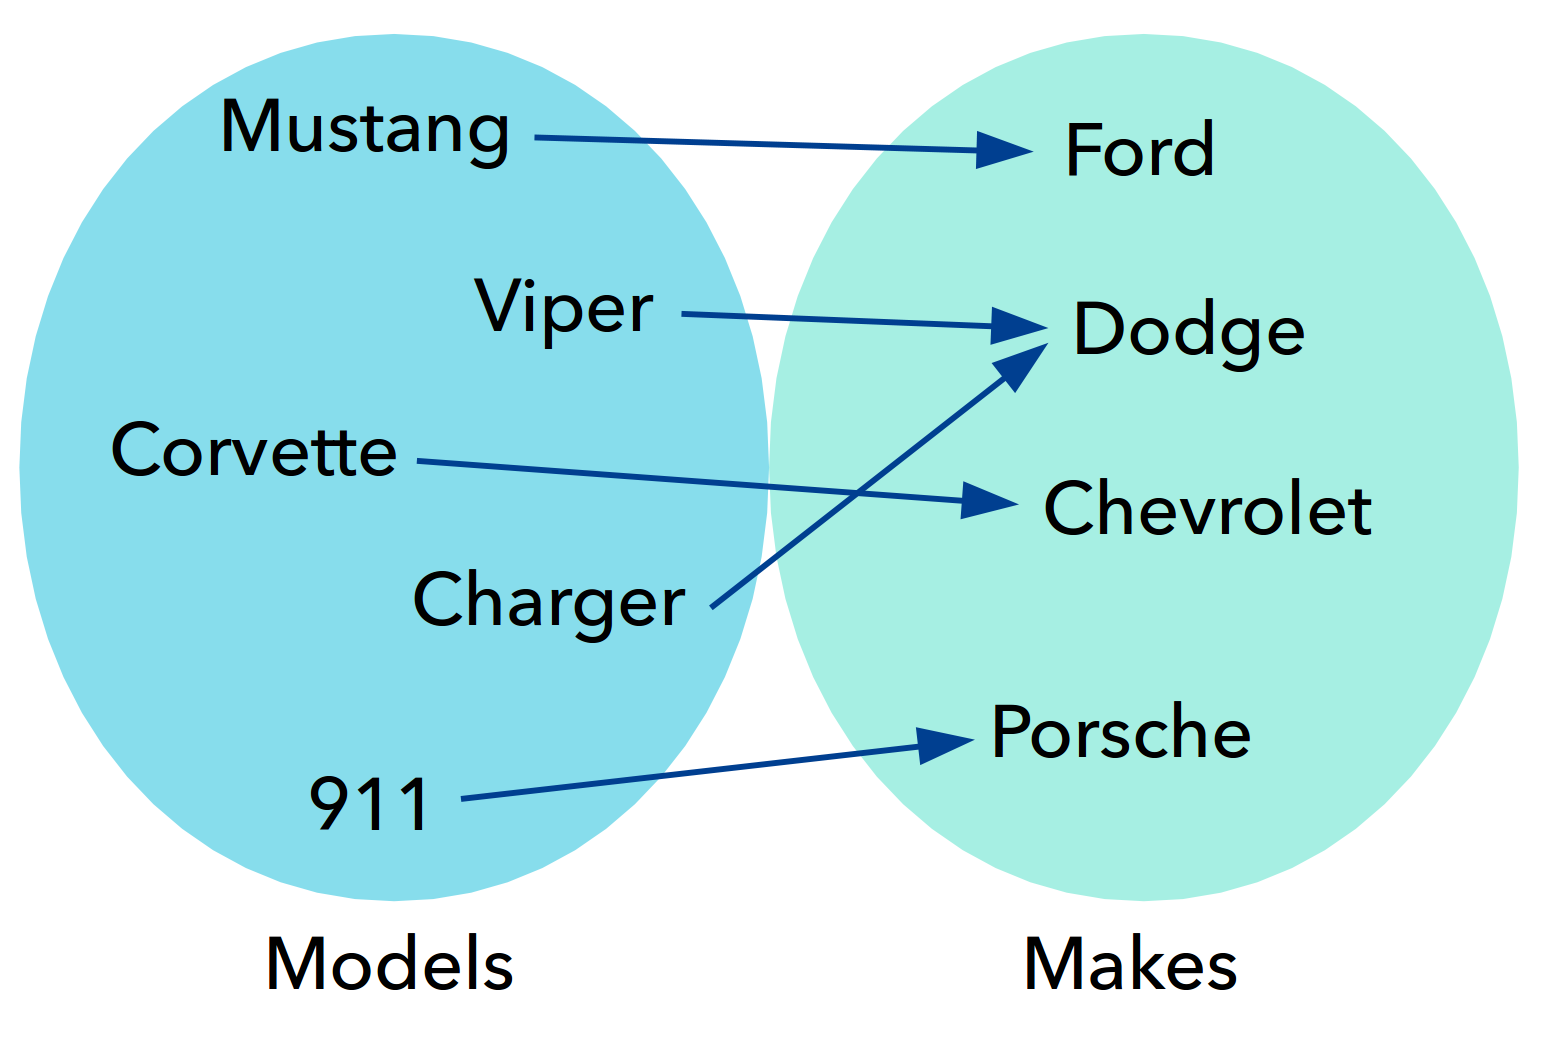
\includegraphics[height=0.75\textheight]{./img/dict-01.png}
\end{frame}

%%%%%%%%%%%%%%%%%%%%%%%%%%%%%%%%%%%%%%%%%%%%%%%%%%%%%%%%%%%%%%%%%%%%%%%%%%%%%%%%
\begin{frame}[fragile]
  \frametitle{\texttt{dict} data type}
  \Enlarge

  \begin{itemize}
  \myitem  The \texttt{dict} indexes data by \emph{any} value (\emph{unordered}). %\pause
  \myitem  Easy to think of as dictionary, but can use lots besides strings. %\pause
  \myitem  This container maps \emph{keys} to \emph{values}. %\pause
  \end{itemize}
  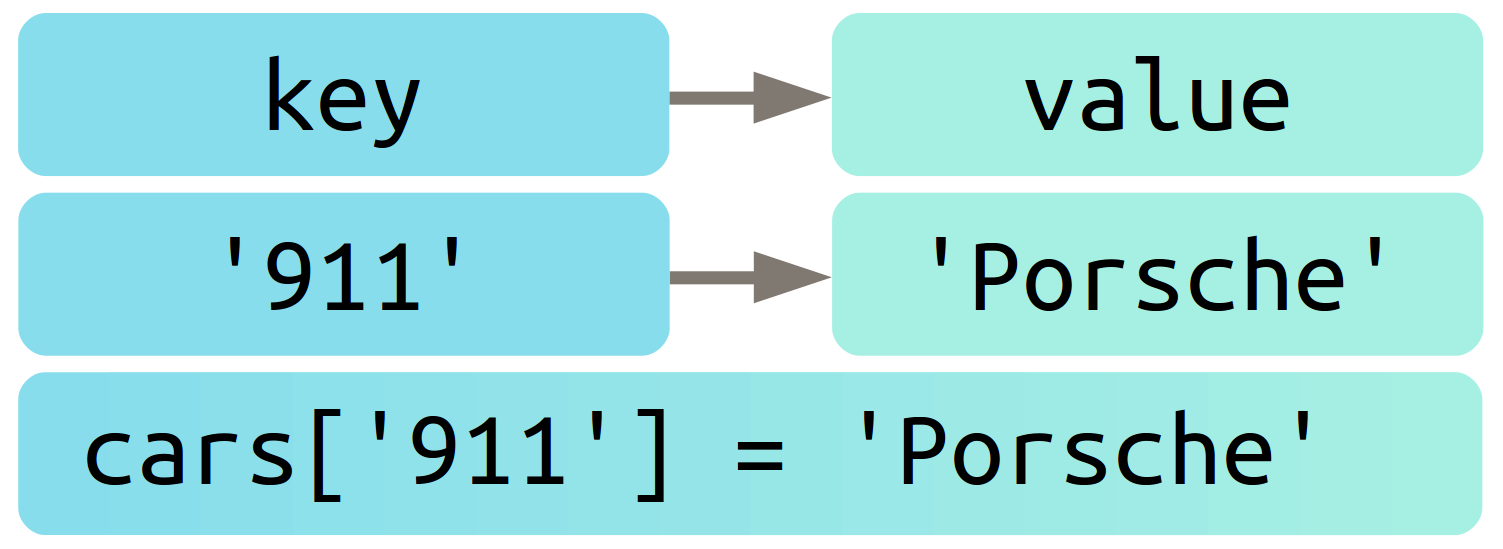
\includegraphics[height=0.333\textheight]{./img/dict-02.png}
\end{frame}

%%%%%%%%%%%%%%%%%%%%%%%%%%%%%%%%%%%%%%%%%%%%%%%%%%%%%%%%%%%%%%%%%%%%%%%%%%%%%%%%
\begin{frame}[fragile]
  \frametitle{\texttt{dict} data type}
  \Enlarge

  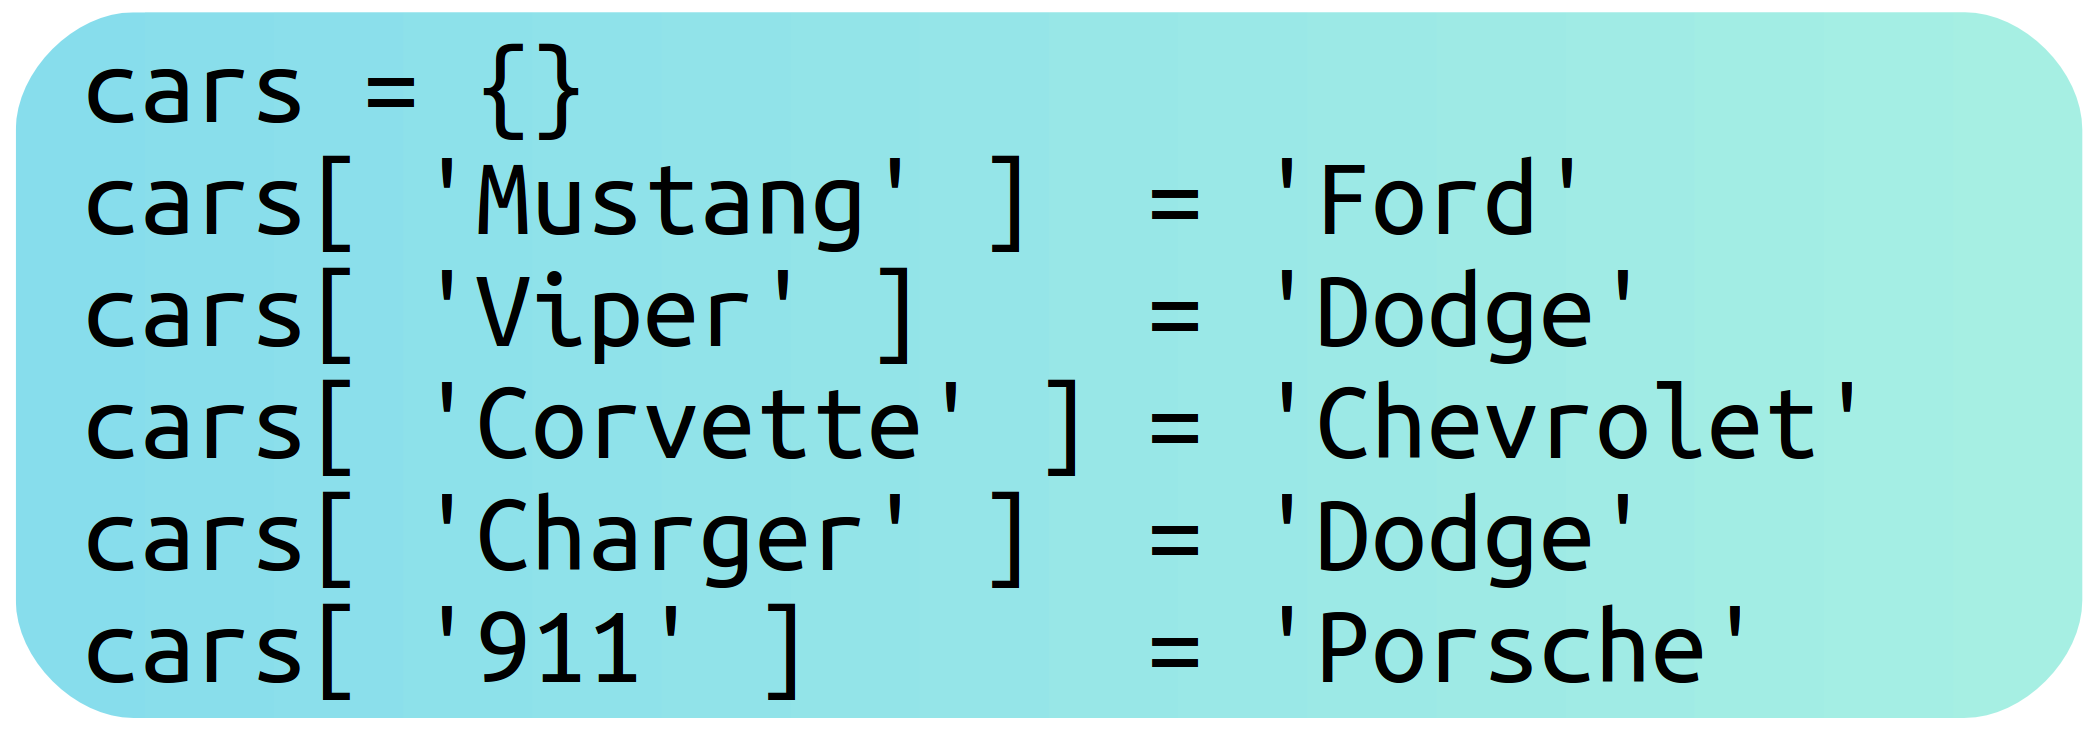
\includegraphics[width=\textwidth]{./img/dict-03.png}
\end{frame}

%%%%%%%%%%%%%%%%%%%%%%%%%%%%%%%%%%%%%%%%%%%%%%%%%%%%%%%%%%%%%%%%%%%%%%%%%%%%%%%%
\begin{frame}[fragile]
  \frametitle{\texttt{dict} literals}
  \Enlarge

  \begin{itemize}
  \myitem  We create a \texttt{dict} as follows:
    \begin{itemize}
    \mysubitem  opening brace \texttt{\{}
    \mysubitem  \texttt{key : value} pairs, separated by commas
    \mysubitem  closing brace \texttt{\}}
    \end{itemize}
  \end{itemize} %\pause
  \begin{semiverbatim}
model = \{
  'Civic': 'Honda',
  'Mustang': 'Ford',
  'Model S': 'Tesla',
  'Model T': 'Ford'
\}
  \end{semiverbatim}
\end{frame}

%%%%%%%%%%%%%%%%%%%%%%%%%%%%%%%%%%%%%%%%%%%%%%%%%%%%%%%%%%%%%%%%%%%%%%%%%%%%%%%%
\begin{frame}[fragile]
  \frametitle{\texttt{dict} operations \& methods}
  \Enlarge

  \begin{semiverbatim}
d = \{ 'one':1, 'two':2, 'three':3 \}
print( d['one'] )
d[ 'four' ] = 4
del d[ 'four' ]
'five' in d
for key in d:  # no guarantee on order
    print( key, d[key] )
d.keys()
d.values()
  \end{semiverbatim}
\end{frame}

%%%%%%%%%%%%%%%%%%%%%%%%%%%%%%%%%%%%%%%%%%%%%%%%%%%%%%%%%%%%%%%%%%%%%%%%%%%%%%%%
\begin{frame}[fragile]
  \frametitle{Example}
  \Enlarge

  \begin{semiverbatim}
d = \{ 'a':2, 'c':3, 'b':1 \}
x = d[ 'a' ] + d[ 'c' ]
  \end{semiverbatim}
  What is the final value of \texttt{x}?
  \begin{enumerate}[label=\Alph*]
  \item  \texttt{4}
  \item  \texttt{'ac'}
  \item  \texttt{'5'}
  \item  \texttt{5}
  \end{enumerate}
\end{frame}

%%%%%%%%%%%%%%%%%%%%%%%%%%%%%%%%%%%%%%%%%%%%%%%%%%%%%%%%%%%%%%%%%%%%%%%%%%%%%%%%
\begin{frame}[fragile]
  \frametitle{Example}
  \Enlarge

  \begin{semiverbatim}
d = \{ \}
words = [ 'red', 'orange', 'yellow' ]
for word in words:
    d[ word ] = words.index( word )
  \end{semiverbatim}
  What is the final value of \texttt{d}?
  \begin{enumerate}[label=\Alph*]
  \item  \texttt{\{ 'red':3, 'orange':6, 'yellow':6 \}}
  \item  \texttt{\{ 'red':0, 'orange':2, 'yellow':2 \}}
  \item  \texttt{None}
  \item  \texttt{\{'orange': 1, 'red': 0, 'yellow': 2\}}  %$\star$
  \end{enumerate}
\end{frame}

%%%%%%%%%%%%%%%%%%%%%%%%%%%%%%%%%%%%%%%%%%%%%%%%%%%%%%%%%%%%%%%%%%%%%%%%%%%%%%%%
\begin{frame}[fragile]
  \frametitle{\texttt{dict} applications}
  \Enlarge

  \begin{itemize}
  \myitem  Dictionaries can encode/decode data, or translate from one representation to another.
  \end{itemize} %\pause
  \begin{semiverbatim}
x = 'ABCDEFGHIJKLMNOPQRSTUVWXYZ'
y = 'BCDEFGHIJKLMNOPQRSTUVWXYZA'
e = \{ \}
for i in range( len(x) ):
    e[ x[i] ] = y[i]
encoded = ''
for c in 'HELLO':
    encoded += e[c]
  \end{semiverbatim}
  \begin{itemize}
  \myitem  How would you reverse (decode) this?
  \end{itemize}
\end{frame}

%%%%%%%%%%%%%%%%%%%%%%%%%%%%%%%%%%%%%%%%%%%%%%%%%%%%%%%%%%%%%%%%%%%%%%%%%%%%%%%%
\begin{frame}[fragile]
  \frametitle{\texttt{dict} applications}
  \Enlarge

  \begin{semiverbatim}
x = 'ABCDEFGHIJKLMNOPQRSTUVWXYZ'
y = 'BCDEFGHIJKLMNOPQRSTUVWXYZA'
d = \{ \}
for i in range( len(x) ):
    d [y[i] ] = x[i]
decoded = ''
for c in encoded:
    decoded += d[c]
  \end{semiverbatim}
\end{frame}

%%%%%%%%%%%%%%%%%%%%%%%%%%%%%%%%%%%%%%%%%%%%%%%%%%%%%%%%%%%%%%%%%%%%%%%%%%%%%%%%
\begin{frame}[fragile]
  \frametitle{Exercise}
  \Enlarge

  \begin{itemize}
  \myitem  Encode all of the words in a file using a Caesar cipher (https://en.wikipedia.org/wiki/Caesar\_cipher).
  \myitem  Decode all of the words in the file.
  \end{itemize}
\end{frame}

%%%%%%%%%%%%%%%%%%%%%%%%%%%%%%%%%%%%%%%%%%%%%%%%%%%%%%%%%%%%%%%%%%%%%%%%%%%%%%%%
\begin{frame}[fragile]
  \frametitle{\texttt{dict} applications}
  \Enlarge

  \begin{itemize}
  \myitem  Dictionaries can also function as accumulators.
  \end{itemize}
  \begin{semiverbatim}
x = 'ABBACAB'
d = \{ \}
for c in x:
    if c not in d:
        d[c] = 0
    d[c] += 1
  \end{semiverbatim}
  \begin{itemize}
  \myitem  How would you reverse (decode) this?
  \end{itemize}
\end{frame}

%%%%%%%%%%%%%%%%%%%%%%%%%%%%%%%%%%%%%%%%%%%%%%%%%%%%%%%%%%%%%%%%%%%%%%%%%%%%%%%%
\begin{frame}[fragile]
  \frametitle{Exercise}
  \Enlarge

  \begin{itemize}
  \myitem  Count category frequencies in Jeopardy questions.
  \myitem  Count bigram frequencies in Jeopardy clues.
  \end{itemize}
\end{frame}

%%%%%%%%%%%%%%%%%%%%%%%%%%%%%%%%%%%%%%%%%%%%%%%%%%%%%%%%%%%%%%%%%%%%%%%%%%%%%%%%
\begin{frame}[fragile]
  \frametitle{\texttt{dict} applications}
  \Enlarge

  \begin{itemize}
  \myitem  We can link data based on a common field.
  \end{itemize}
  \begin{semiverbatim}
zipcode = \{ 'Bill': 60644,
            'Jill': 41073,
            'Tony': 63103 \}
city = \{ 60644: 'Chicago',
         41073: 'Cincinnati',
         63103: 'St. Louis' \}
for name in zipcode:
    print( name,city[ zipcode[ name ] ] )
  \end{semiverbatim}
\end{frame}

%%%%%%%%%%%%%%%%%%%%%%%%%%%%%%%%%%%%%%%%%%%%%%%%%%%%%%%%%%%%%%%%%%%%%%%%%%%%%%%%
\section{Mutable Arguments}

%%%%%%%%%%%%%%%%%%%%%%%%%%%%%%%%%%%%%%%%%%%%%%%%%%%%%%%%%%%%%%%%%%%%%%%%%%%%%%%%
\begin{frame}[fragile]
  \frametitle{Exercise:  mutability}
  \Enlarge

  \begin{semiverbatim}
x = [ 3,2,1 ]
y = x
y.sort()
x.append( 0 )
  \end{semiverbatim}
  What is the final value of \texttt{x}?
  \begin{enumerate}[label=\Alph*]
  \item  \texttt{[ 3,2,1 ]}
  \item  \texttt{[ 1,2,3 ]}
  \item  \texttt{[ 1,2,3,0 ]} % $\star$
  \item  \texttt{[ 0,1,2,3 ]}
  \end{enumerate}
\end{frame}

%%%%%%%%%%%%%%%%%%%%%%%%%%%%%%%%%%%%%%%%%%%%%%%%%%%%%%%%%%%%%%%%%%%%%%%%%%%%%%%%
\begin{frame}[fragile]
  \frametitle{Mutable arguments}
  \Enlarge

  \begin{itemize}
  \myitem  Mutability causes \texttt{list}s to work differently in functions. %\pause
  \myitem  \texttt{list}s used as arguments \emph{can be changed} by the function. %\pause
  \myitem  This is very useful! %\pause
  \end{itemize}
  \begin{semiverbatim}
def fun(q):
    q.append(3)

a = [ ]
for i in range(3):
    fun(a)
print(a)
  \end{semiverbatim}
\end{frame}

%%%%%%%%%%%%%%%%%%%%%%%%%%%%%%%%%%%%%%%%%%%%%%%%%%%%%%%%%%%%%%%%%%%%%%%%%%%%%%%%
\begin{frame}[fragile]
  \frametitle{Mutable arguments}
  \Enlarge

  \begin{semiverbatim}
def readfile(fname,a):
    for line in open(fname):
        a.append(line)

all_lines = []
readfile( 'file1.txt', all_lines )
readfile( 'file2.txt', all_lines )
  \end{semiverbatim}
\end{frame}

%%%%%%%%%%%%%%%%%%%%%%%%%%%%%%%%%%%%%%%%%%%%%%%%%%%%%%%%%%%%%%%%%%%%%%%%%%%%%%%%
\begin{frame}[fragile]
  \frametitle{Mutable arguments}
  \Enlarge

  \begin{semiverbatim}
def readfile(fname,a):
    for line in open(fname):
        a.append(line)

all_lines = [ ]
for f in open( "filenames.txt" ):
    readfile( f,all_lines )
  \end{semiverbatim}
\end{frame}

%%%%%%%%%%%%%%%%%%%%%%%%%%%%%%%%%%%%%%%%%%%%%%%%%%%%%%%%%%%%%%%%%%%%%%%%%%%%%%%%
\begin{frame}[fragile]
  \frametitle{Copying mutable values}
  \Enlarge

  \begin{itemize}
  \myitem  What if we \emph{want} a copy of a \texttt{list} (not an alias)? %\pause
  \myitem  Slice everything! %\pause
  \end{itemize}
  \begin{semiverbatim}
x = [ 3,2,1 ]
y = x[ : ]
y.sort()
print( x )
  \end{semiverbatim}
\end{frame}

%%%%%%%%%%%%%%%%%%%%%%%%%%%%%%%%%%%%%%%%%%%%%%%%%%%%%%%%%%%%%%%%%%%%%%%%%%%%%%%%
\begin{frame}[fragile]
  \frametitle{Copying mutable values}
  \Enlarge

  \begin{semiverbatim}
x = [ 1,2,3 ]
y = x[ : ]
y.append( 4 )
print( x == y )
  \end{semiverbatim}
\end{frame}

%%%%%%%%%%%%%%%%%%%%%%%%%%%%%%%%%%%%%%%%%%%%%%%%%%%%%%%%%%%%%%%%%%%%%%%%%%%%%%%%
\begin{frame}[fragile]
  \frametitle{\texttt{is} tests identity}
  \Enlarge

  \begin{semiverbatim}
a = [ 1,2,3 ]
b = a
c = a[ : ]

b is a  # True
c is a  # False
  \end{semiverbatim}
\end{frame}

%%%%%%%%%%%%%%%%%%%%%%%%%%%%%%%%%%%%%%%%%%%%%%%%%%%%%%%%%%%%%%%%%%%%%%%%%%%%%%%%
\section{Reminders}

%%%%%%%%%%%%%%%%%%%%%%%%%%%%%%%%%%%%%%%%%%%%%%%%%%%%%%%%%%%%%%%%%%%%%%%%%%%%%%%%
\begin{frame}
  \frametitle{Reminders}
  \Enlarge

  \begin{itemize}
  	\myitem  Homework \#5 is due Wed Nov.\ 9.
  	\myitem  Midterm \#1 will be Monday Nov.\ 7, 7pm-9pm.  (evening) in A-0414\\ \textcolor{CS101GradBot}{No lecture on Nov. 7 Monday but the instructor is available for office hour during the lecture time in Office 410 Arts and Science Building.}
  \end{itemize}
\end{frame}

\end{document}
